
\section{Supervised Learning}\label{sec:supervised-learning}
There are several supervised learning~\ref{subsec:supervised-and-unsupervised-learning-methods} bot detection schemes that utilize labeled datasets to train models in their implementation.

\subsection{Deep Learning with Mouse Behavior Metrics}\label{subsec:deep-learning-with-mouse-behavior}
The detection scheme described in~\cite{deep_learning_detection_with_mouse_behavior} analyzes the mouse movement and operations of a user to decide whether these gestures are consistent with that of a human user or bot user.
Images containing the spatial and kinetic information that represents the mouse behavioral metrics are passed into a deep neural network for making the bot or not decision.
Representing the models in such a way has enabled the use of a Convolutional Neural Network, or "CNN", to automate feature learning from a user's raw mouse position data.

Rather than following the patterns of previous implementations that fed hand-crafted features into shallow machine learning models, this work transforms every mouse movement sequence into a separate image that contains the spatial and kinetic information about the mouse positions and movements.
By doing so, CNN models can be used in this deep learning approach.
Related detection schemes that utilize mouse behavioral metrics most likely use statistics of mouse movement sequences as a means to create features.
Some of these features, common to this thesis work, include the mean, median, or variance of velocities, accelerations, etc.
As an improvement from this trend, the said work contributes to the field by proposing a method of more accurately representing shape information of the user's mouse movement trajectories.
This is an underlying motivation to use CNNs, since the complexities of these mouse trajectories can not be represented by using common statistical metrics.

The architecture of this deep learning approach allows for decisions of a user's botness, meaning if they are a bot or not, in a realtime setting.
\begin{figure}[!h]
    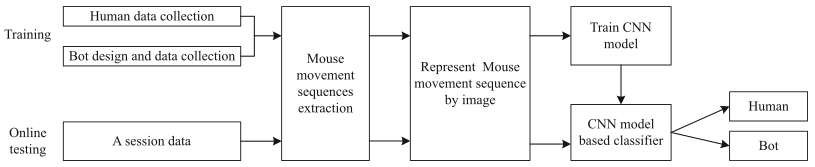
\includegraphics[width=1\columnwidth]{figures/deep_learning_with_mouse_dynamics_system_architecture}
    \caption{Architecture of the deep learning model using CNNs}
    {\small System design from the research in~\cite{deep_learning_detection_with_mouse_behavior}}
    \label{fig:deep-learning-architecture}
\end{figure}
A user's botness is determined by considering the classification results of most mouse movement sequences extracted from the operation data created at the left-most, first stage of the architecture diagram.
Therefore, if the classifier depicts inputted mouose movement sequences to be that of a bot, than that particular user, or source of raw mouse position data, will be classified as a bot.
A few metrics were created to represent a user's mouse movement behavior:
\begin{itemize}
    \item \textbf{mouse movement sequence}: the records of a series of consecutive mouse moves
    \item \textbf{mouse trajectory}: a time-space curve corresponding to a mouse movement sequence
    \item \textbf{step size}: the distance between two consecutive points
    \item \textbf{event interval}: the time difference between two points
\end{itemize}
Similarly to this thesis research, the \textbf{mouse movement sequence}s are in the format $(x_i, y_i, t_i)$, where $i = 1{\dots}n$ with $n$ being the number of mouse positions in the sequence, $x$ and $y$ are the 2D coordinates of a mouse cursor's position, and $t$ is the time of when that cursor was at the respective position.

Representing a user's mouse movements is done by separating the continuous sequences of mouse events into segments of sequences that correspond to individual mouse movements.
Their assumption is that the intervals between mouse events does not exceed 100ms.
This closely aligns with the average mouse position polling rate of 125hz~\cite{mouse_dpi_and_polling_rate_explained}~\cite{mouse_dpi_and_usb_polling_rate}.
Any mouse movement sequence segments containing less that 15 events were discarded, as these events were said to not contain enough information for bot detection.
Following this sequence segmentation stage, a two-step process was implemented to transform the mouse movement sequence segments into images that can be used in the CNN model.

\textbf{Mapping spatial information into the image} was achieved by using shape and distance metrics between consecutive events of a segment.
The images were centered by finding the halfway point of the max distance between any two points in the segment.
Zoom was considered since the max distances vary among different segments.
With this in mind, all mouse positions in the segements were set to a constant 8px diameter.
\textbf{Mapping kinetic information into the image} was achieved by reflecting the event interval series and step size series.
The paper's denotations for these were $({\Delta}t_1,\dots,{\Delta}t_{n-1})$ and $({\Delta}d_1,\dots,{\Delta}d_{n-1})$ respectively.
In short, they used velocity as the feature to be represented in the images.
Every point in the segments were color-coded based on the magnitude of velocity calculated at each point.
The colors were on the red, blue, green (RGB) scale, and decided by mapping the delta values to an integer ranging from 0 to 255.
\begin{figure}[!h]
    \centering
    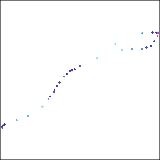
\includegraphics[width=.35\columnwidth]{figures/deep_learning_with_mouse_dynamics_mouse_segment_image_generation}
    \caption{Conversion of a mouse sequence segment to an image}
    \label{fig:deep-learning-image-generation}
    {\small Spatial and kinetic information of a users mouse movement behavior are represented in images similar to this one, as shown in~\cite{deep_learning_detection_with_mouse_behavior}. The mouse positions of mouse movement are shown in each sequence segment, a single image, and colors denote the velocity of mouse movement.}
\end{figure}
Bot users, specifically, were fabricated by 4 different types of bot scripts, each generating a unique pattern to their mouse movement trajectories.
Figure~\ref{fig:deep-learning-image-generation-bots} displays images that represent these 4 types.
\begin{figure}[!h]
    \centering
    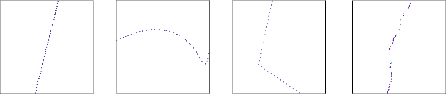
\includegraphics[width=1\columnwidth]{figures/deep_learning_with_mouse_dynamics_mouse_segment_image_generation_bots}
    \caption{Conversion of bot mouse sequence segments to an image}
    \label{fig:deep-learning-image-generation-bots}
    {\small Shown are examples of the 4 different types of bot mouse trajectories: \textit{straight-line}, \textit{curve}, \textit{polyline}, and \textit{semi-straight line}, respectively, as shown in~\cite{deep_learning_detection_with_mouse_behavior}}
\end{figure}
The semi-straight line was created by adding noise to the points on the straight-line mouse trajectory.
Bezier curves were used to make the curve and polyline trajectories.
All mouse sequence segments were created with a few different intervals between mouse events.
These intervals were added by either a set constant value, uniformly distributed values, or values with a Gaussian distribution.
Human datasets were gathered over a 2 month period of recording the activity of several human users.
With these datasets, images were generated in the manner previously described, thus allowing for a supervised learning, CNN model approach.
Although this paper reflects 90-99\% detection accuracy for all 4 types of bots, their results may reflect a testing bias.
Since the authors of this paper implemented the bot datasets, their methods of detecting said bots may cause testing biased to their own implementations, thus skewing results.

\subsection{Graphs and CNNs}\label{subsec:graphs-and-cnns}
BotGraph\cite{botgraph} is one which represented the sitemap, or order of page indexing, of a user with a nodes-and-edges graph.
Since these generated graphs are images that represent a number of metrics based on user behavior, not user identification, the research utilized CNNs to predict users types of either bot or human.
The BotGraph research concludes that this approach yields about a 95\% success rate in detecting bots.

This article begins by introducing key concepts mentioned by a company that specializes in web bot detection, ShieldSquare, the difference of identity-based and behavior-based bot detection.
The identify-based method utilizes client-side JavaScript to collect parameters like browser fingerprints; a collection of information about your browser type and version, as well as your operating system, active plugins, timezone, language, screen resolution and various other active settings~\cite{browser_fingerprinting}.
Whereas behavior-based methods utilize the number pages visited per session, the duration of time per page visit, and the number of page revisits, etc.
This research more closely resembles the behavior-based method but instead represents such metrics via a graph image which, according to the research, contains more unique features per user.
The paper continues by introducing a violator blacklist, biometric data validation like scroll and mouse movement method by Distil Networks, as well as the UserAgent variable present in HTTP protocol; an unstable bot-detection method as more advanced bots can falsify their identity by simply hiding or modifying the UserAgent variable.
DeepDefense~\cite{deep_defense_article} introduced a recurrent neural network (RNN)-based model that takes as input same-shape segment splits from the web server access logs, then encoded the request information in each line of segment to a numerical matrix.
The paper states that, while this method is most similar to the outlined research implementation, the inference efficiency of Deep Defense relies too heavily on the length of the same-shape segments; in which BotGraph supposedly proves to be more stable.

The research implementation included BotGraph, a program that generates graph-based representations of users' sitemap traversals.
Since these graphs were in image format, the implementation employed convolutional neural network (CNN) inferences to distinguish bots from human user types.
The details of BotGraph are as follows:
\begin{itemize}
    \item request - timestamp, HTTP method, request URI, status, host IP, user{\_}agent, client IP variables
    \item session - a method if identifying a series of client requests (by bot or human)
    \item identity - user{\_}agent and client IP variables for the client, and host IP variable for the server
    \item behavior - request URI and status variables for the access frequency metric per graph node.
\end{itemize}
The graph can be described as $G = (V, E)$:
\begin{itemize}
    \item $G$: a directed graph
    \item $V$: set of nodes representing all same-pattern URLs visited, i.e \textbf{/page?id=3} is pattern \textbf{/page?id=*}
    \item $E$: set of directed edges, each representing access points, i.e. \textbf{\textit{a}} tag elements with same href
\end{itemize}
Below is a figure of the BotGraph architecture. As you can see, BotGraph runs in a three-step process:
\begin{enumerate}
    \item Build a sitemap through one of three methods: \textit{active crawling, passive sniffing, self providing}
    \begin {enumerate}
        \item \textit{active crawling}: crawling typically starts from website homepage and recursively enters each hyperlink from the current page
        \item \textit{passive sniffing}: a website’s traffic is monitored, learned then used to build the sitemap. This is a less intrusive alternative to active crawling
        \item \textit{self providing}: the site provides its own sitemap for bot detection. This is the most accurate
    \end{enumerate}
    \item Map requests listed in server access logs to denote sessions as subgraphs in a sitemap
    \item Generate 2-dimensional trace images, translating a bot detection task into an image recognition
\end{enumerate}
\begin{figure}[!h]
    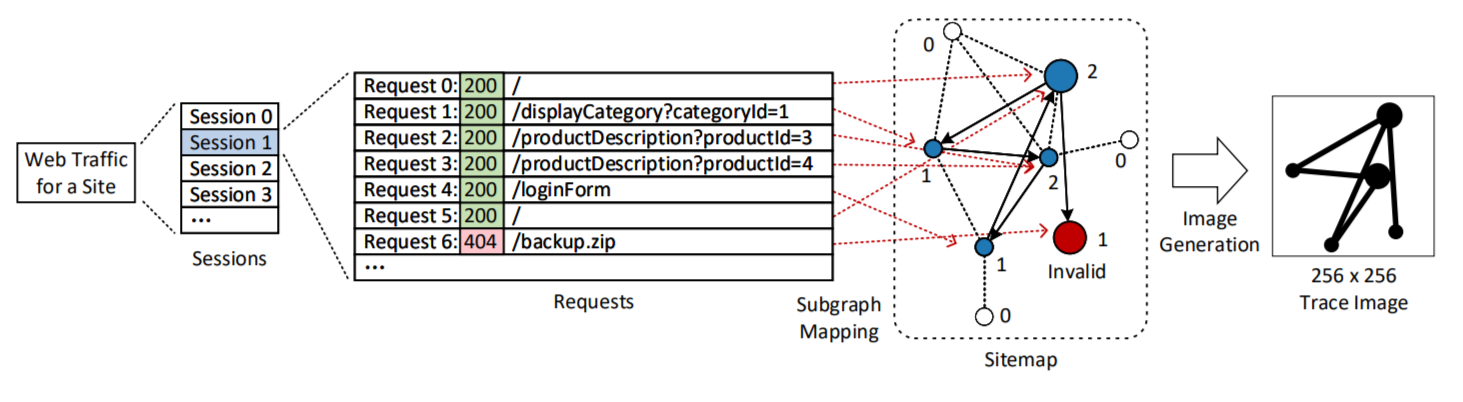
\includegraphics[width=1\columnwidth]{figures/BotGraph_fig1}
    \caption{Architecture of BotGraph}
    {\small Diagram from BotGraph~\cite{botgraph}}
    \label{fig:botgraph}
\end{figure}
This implementation used a model trained on a data set generated by 30+ professionals that manually tagged web traffic via JavaScript support checking, mouse movement and click tracking, IP reputation, UserAgent blacklisting.

A weakness in the BotGraph method of bot detection is when a user visits a lower number pages per session, i.e. less than 3 visits.
This is because bot and human users have too similar browsing behavior, namely their session sitemap traversal, creating near-identical sitemap graphs.
However, this research claims that BotGraph is a very effective and efficient method of detecting bots as it achieves about 95\% in precision and recall while relying only on the client's behavior and not the client's identity variables.
Some needed improvements include an implementation that generates more detailed graph-related features to better describe the characteristics of user sessions, specifically to identify the behavior of web bots.

\subsection{Training Data Generation and Semi-Supervised Learning}\label{subsec:training-data-generation-and-semi-supervised-learning}
The research described in~\cite{bot_detection_for_search_engines} addresses the common problem with supervised learning-based bot detection schemes.
Due to the high traffic of modern search engines, it is infeasible to rely on human judges to generate labeled datasets, used in supervised learning approaches, by manually inspecting the search logs to label bot and human users.
On a controlled webserver environment, labeled datasets were created by analyzing the response and activity of CAPTCHA challenges sent to the users.
In an effort to enhance the user experience, challenges were sent selectively, either when the webserver is experiencing a high volume of network traffic, or when a user makes a high number of requests in a short amount of time.
When presented with a challenge, the user can either disregard the challenge by exiting the session, answer correctly, or answer correctly, thus answering "no response", "correct response", or "wrong response", respectively.
\begin{figure}[!h]
    \centering
    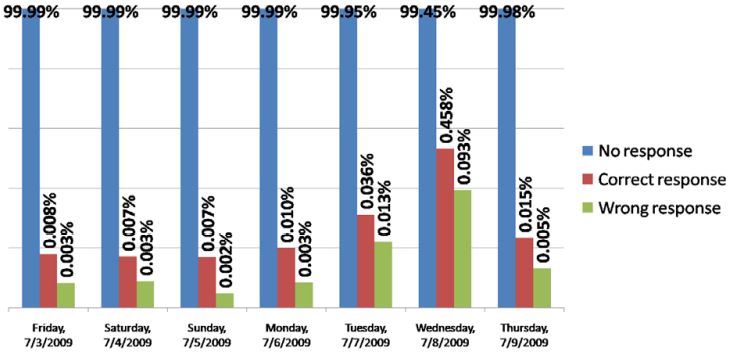
\includegraphics[width=1\columnwidth]{figures/semi_supervised_CAPTCHA_training_data_generation_results}
    \caption{User answers to CAPTCHA challenges}
    \label{fig:captcha-user-answers}
    {\small The research notes that since the users were selected non-uniformly, most answers to the challenge were "no response", as shown in~\cite{bot_detection_for_search_engines}}
\end{figure}
About 80\% of the received responses were correct.
This accounted for the majority of the training data with "human" labels.
The remaining "human" labels were pulled from the large set of "no response" answers by analyzing heuristics of the user's number of clicks in a time period, the number of search result pages browsed, as well as information of the user's IP address.
Users were labeled "bot" if the user's answer was "no response", and the user did not satisfy thresholds of the heuristics previously described.
This CAPTCHA challenge-method accounted for the "0-cost" training data generation method, as described in the research.

From the creation of the labeled training dataset, the following features were extracted from the users:
\begin{itemize}
    \item \textbf{PageTrackedCount}: measures the number of pages that the user browses
    \item \textbf{UserClickCount}: measures the number of mouse clicks on the search result pages
    \item \textbf{AllHitCount}: measures the overall "impressions" that the user receives in addition to the search results
    \item \textbf{UserUniqueIPs}: measures the unique number of IPs a user is using
    \item \textbf{UserUniqueQueries}: measures the unique number of queries issued by a single user in a search session
    \item \textbf{Blacklisting Rules}:
    \begin{enumerate}
        \item \textbf{Form}: triggered when a user includes in the query certain obscure codes that are designed mostly for internal search engine instrumentation purposes that should be unfamiliar to most genuine human users
        \item \textbf{IP}: a list of IPs that are publicly identified as Internet spammers and labeled all the traffic from these IPs as "bot"
        \item \textbf{Query}:  this rule is triggered when the query composition is too complicated to be manually typed in by a human user
    \end{enumerate}
\end{itemize}
The research stated, regarding the \textbf{PageTrackedCount}, that bots tend to behave in two extremes.
Some bots will only submit queries and not browse any of the result pages (except the first one), ostensibly with the intention to increase the query frequency for certain keywords.
The other extreme sees the bots fetch all the result pages for each query, probably trying to reverse engineer the index of the search engine, while genuine human users would probably just browse the first few pages of the query results selectively.
For \textbf{UserClickCount}, clicks on the search engine results, as well as clicks on advertisements within the results, were included in the click counts.
The research noted that the advertisement clicks, though are not distinguished in this work, may include bots specifically targeting ads to click.

With these features, a supervised learning method of bot detection was used.
In said research, the C4.5~\cite{c4.5} algorithm was the decision tree used in lieu of a custom implementation, stating "details of the decision tree algorithm are omitted here".
By leveraging the autonomously created labeled training dataset, sourced from CAPTCHA response and filtered by following the previously mentioned heuristics, the decision tree algorithm was projected to work well.
However, despite the positive projections, the results have shown to be inconsistent from the true data distribution, begging the question of the classification's integrity.
This may be a result of the training dataset generation stage, since the "bot" labels are subject to the heuristics determined by domain experts.
A useful approach to this dilemma was their statistical method of using numerous unlabeled data, due to uncertainties in the "0-cost" training data generation.
Despite the evaluated performance improvement from the tested supervised learning approach, some inconsistencies would need to be addressed in future work.
Due to the limited time of one week to present CAPTCHA challenges to users, some search engine bots may have been undetected, thus diminishing the integrity of the training data generation.
Therefore, it is unclear if this bot detection scheme can be as useful during more real, long-term scenarios.
